

\fancypagestyle{miEstilo2}{
   \lhead{2. Planificación}
   %\chead{1. Introducción}
   \rhead{Página \thepage}
   \lfoot{}
   \cfoot{}
   \rfoot{}
}

\pagestyle{miEstilo2}

\section{Planificación}

Como en todo proyecto, realizar una buena planificación es la clave para no fracasar en el desarrollo del mismo. Por ello, se ha realizado una planificación detallada del proyecto, utilizando los conceptos de \textit{iteraciones} y \textit{sprints} para ir distribuyendo el trabajo a lo largo de las semanas, durante las cuales se han ido desarrollando una serie de tareas que cumplen un objetivo específico.

Estos conceptos surgen de los llamados métodos de desarrollo ágiles, en los cuales se intenta descomponer una aplicación o proyecto por funcionalidades, y el objetivo es ir desarrollando y testeando cada una de forma independiente para poder integrarla con el resto.

La planificación que se ha previsto para el desarrollo del proyecto es la siguiente:

\begin{table}[h!]
\centering
\begin{tabular}{|p{5cm}|p{4cm}|}
 \hline
	\cellcolor[gray]{0.9} Número de semanas  & 11\\ \hline
	\cellcolor[gray]{0.9} Tiempo total estimado (h)  & 341h \\ \hline
	\cellcolor[gray]{0.9} Fecha de inicio del proyecto  & 01-07-2019 \\ \hline
	\cellcolor[gray]{0.9} Fecha de fin del proyecto  & 15-09-2019 \\ \hline
		
\end{tabular}
\end{table}

\subsection{Fase preparatoria}

En esta fase se comenzará el desarrollo del proyecto, que tiene un esfuerzo estimado de \textbf{36.5 horas}. Se realizará un estudio de viabilidad de la idea del proyecto, así como un estudio de mercado, una investigación acerca de las posibles herramientas a usar \ldots.

El objetivo de esta primera fase es tener claro que el proyecto es viable tanto en recursos, tiempo y presupuesto, para que posteriormente comience su desarrollo e implementación.


% ###########################  ITERACIÓN 1   ###########################

\large{\underline{\textbf{Iteración 1}: Análisis y estudio de la aplicación.}}
\vspace{0.3cm}

\normalsize

En esta iteración se describirán los principales objetivos de la aplicación, se estudiará sus posibles casos de uso y se elaborará un plan de iteraciones para planificar el desarrollo del proyecto a lo largo del tiempo que se dispone.

Para esta iteración, se ha establecido la siguiente planificación:

\begin{table}[h!]
\centering
\begin{tabular}{|p{5cm}|p{4cm}|}
 \hline
	\cellcolor[gray]{0.9} Semana  & 1\\ \hline
	\cellcolor[gray]{0.9} Tiempo total previsto (h)  & 36.5h \\ \hline
	\cellcolor[gray]{0.9} Fecha de inicio  & 01-07-2019 \\ \hline
	\cellcolor[gray]{0.9} Fecha de fin  & 06-07-2019 \\ \hline
		
\end{tabular}
\end{table}

Esta iteración consta de los siguientes sprints:

\textbf{Sprint 1}: Descripción de la aplicación


\begin{table}[h!]
\begin{tabular}{|p{4cm}|p{7.2cm}|p{1.3cm}|p{2.1cm}|}
\hline
\rowcolor[HTML]{9B9B9B} 
{\color[HTML]{FFFFFF} Product backlog} & {\color[HTML]{FFFFFF} Descripción}                                  & {\color[HTML]{FFFFFF} Semana} & {\color[HTML]{FFFFFF}Tiempo (h)} \\ \hline
Objetivos                              & Descripción de los objetivos .                                       & 1                             & 0.5                                    \\ \hline
Funcionalidades                        & Descripción de las funcionalidades.                                 & 1                             & 1.5                                    \\ \hline
Motivaciones                           & Motivaciones personales acerca de la temática del proyecto.          & 1                             & 0.5                                    \\ \hline
Usuarios y escenarios                  & Descripción de los posibles casos de uso de la aplicación propuesta. & 1                             & 2                                      \\ \hline
\end{tabular}
\end{table}

\textbf{Sprint 2}: Investigación y preparación del entorno.

\begin{table}[h!]
\begin{tabular}{|p{4cm}|p{7.2cm}|p{1.3cm}|p{2.1cm}|}
\hline
\rowcolor[HTML]{9B9B9B} 
{\color[HTML]{FFFFFF} Product backlog} & {\color[HTML]{FFFFFF} Descripción}                                  & {\color[HTML]{FFFFFF} Semana} & {\color[HTML]{FFFFFF}Tiempo (h)} \\ \hline
Estudio y análisis de mercado                             & Búsqueda de proyectos similares y estudio sobre sus componentes.
                                        & 1                             & 5                                    \\ \hline
Tecnologías y herramientas                        & Estudio de tecnologías y herramientas necesarias para el desarrollo del proyecto.
                                  & 1                             & 5                                   \\ \hline
Entorno de trabajo                          & Creación del repositorio de Github y entorno de desarrollo del proyecto.
          & 1                             & 4                                   \\ \hline
\end{tabular}
\end{table}

\newpage

\textbf{Sprint 3}: Planificación y plan de iteración.


\begin{table}[h!]
\begin{tabular}{|p{4cm}|p{7.2cm}|p{1.3cm}|p{2.1cm}|}
\hline
\rowcolor[HTML]{9B9B9B} 
{\color[HTML]{FFFFFF} Product backlog} & {\color[HTML]{FFFFFF} Descripción}                                  & {\color[HTML]{FFFFFF} Semana} & {\color[HTML]{FFFFFF}Tiempo (h)} \\ \hline
Descomposición de tareas                             & Identificación de funcionalidades y descomposición en tareas.
                                        & 1                             & 4                                   \\ \hline
Plan de iteración                        & Elaboración de un plan de iteración para distribuir todas las tareas a lo largo del tiempo previsto para el desarrollo del proyecto.
                                  & 1                             & 10                                  \\ \hline
Documento de planificación                          & Documento donde se describe el plan de iteración y planificación.
          & 1                             & 4                                   \\ \hline
\end{tabular}
\end{table}


\subsection{Fase de implementación y pruebas}

Una vez se tienen claros los objetivos del proyecto, se ha visto que el proyecto es viable, y se han preparado las principales herramientas a utilizar, comienza la fase de implementación del proyecto.

El objetivo de esta fase es llevar a cabo la idea general del proyecto, es decir, implementar un sistema que sea capaz de realizar las acciones deseadas.

Esta fase de implementación se ha distribuido en varias iteraciones, con el fin de organizar y realizar una parte de la funcionalidad de la aplicación en cada iteración, donde se implementa, prueba y verifica el estado del software.

Al final de esta fase, se habrá obtenido un software implementado incrementalmente, donde se ha testeado cada módulo, tanto con pruebas unitarias como de integración y validación.

Para esta fase, se ha previsto un total de \textbf{221 horas}, y se ha distribuido en las siguientes iteraciones:

\newpage

% ###########################  ITERACIÓN 2   ###########################

\large{\underline{\textbf{Iteración 2}: Implementación de los módulos principales.}}
\vspace{0.3cm}

\normalsize

El objetivo de esta iteración es la implementación de los principales módulos de los que va a constar la aplicación. Estos módulos interaccionarán directamente con el hardware, y/o serán utilizados por los agentes y la API.

Para esta iteración, se ha establecido la siguiente planificación:

\begin{table}[h!]
\centering
\begin{tabular}{|p{5cm}|p{4cm}|}
 \hline
	\cellcolor[gray]{0.9} Semana  & 2\\ \hline
	\cellcolor[gray]{0.9} Tiempo total previsto (h)  & 45h \\ \hline
	\cellcolor[gray]{0.9} Fecha de inicio  & 07-07-2019 \\ \hline
	\cellcolor[gray]{0.9} Fecha de fin  & 14-07-2019 \\ \hline
		
\end{tabular}
\end{table}

\begin{table}[h!]
\begin{tabular}{|p{4cm}|p{7.2cm}|p{1.3cm}|p{2.1cm}|}
\hline
\rowcolor[HTML]{9B9B9B} 
{\color[HTML]{FFFFFF} Product backlog} & {\color[HTML]{FFFFFF} Descripción}                                  & {\color[HTML]{FFFFFF} Semana} & {\color[HTML]{FFFFFF}Tiempo (h)} \\ \hline
Formación                             & Estudio de las bibliotecas de Python necesarias: \textit{PiCamera}, \textit{logging} \ldots
                                        & 2                             & 7                                   \\ \hline
Módulo cámara                        & Implementación del módulo que va a conectar y utilizar la cámara de la raspberry.
                                  & 2                             & 7                                  \\ \hline
Módulo vídeo                          & Implementación del módulo vídeo para conectar y utilizar la cámara de la raspberry.
          & 2                             & 8                                   \\ \hline
Módulo logging                         & Implementación del módulo logging para almacenar todos los logs producidos por módulos, agentes y la \textit{API}.
          & 2                             & 8                                   \\ \hline

Test unitarios                         & Implementación de los test unitarios de los módulos desarrollados en esta iteración y depuración necesaria. & 2 & 15 \\ \hline  

\end{tabular}
\end{table}

\newpage

% ###########################  ITERACIÓN 3   ###########################

\large{\underline{\textbf{Iteración 3}: Implementación de la API principal.}}
\vspace{0.3cm}

\normalsize

El objetivo de esta iteración es la implementación de la API que conectará los distintos módulos de la aplicación y responderá a todas las peticiones que reciba. Adicionalmente, se implementarán tareas asíncronas para evitar posibles esperas y poder atender el máximo número de peticiones simultáneamente.

Para esta iteración, se ha establecido la siguiente planificación:

\begin{table}[h!]
\centering
\begin{tabular}{|p{5cm}|p{4cm}|}
 \hline
	\cellcolor[gray]{0.9} Semana  & 3-4 \\ \hline
	\cellcolor[gray]{0.9} Tiempo total previsto (h)  & 50h \\ \hline
	\cellcolor[gray]{0.9} Fecha de inicio  & 15-07-2019 \\ \hline
	\cellcolor[gray]{0.9} Fecha de fin  & 24-07-2019 \\ \hline
		
\end{tabular}
\end{table}

\begin{table}[h!]
\begin{tabular}{|p{4cm}|p{7.2cm}|p{1.3cm}|p{2.1cm}|}
\hline
\rowcolor[HTML]{9B9B9B} 
{\color[HTML]{FFFFFF} Product backlog} & {\color[HTML]{FFFFFF} Descripción}                                  & {\color[HTML]{FFFFFF} Semana} & {\color[HTML]{FFFFFF}Tiempo (h)} \\ \hline
Formación                             & Estudio de las bibliotecas de Python necesarias: \textit{flask}, \textit{celery}, \textit{requests}, servicio \textit{rabbit mq} \ldots
                                        & 3                             & 8                                   \\ \hline
API                        & Implementación de las funciones principales de la \textit{API}.
                                  & 3                             & 12                                  \\ \hline
Tareas asíncronas                         & Implementación de las tareas asíncronas de la \textit{API}.
          & 3                             & 6                                   \\ \hline
Test unitarios                         & Implementación de los test unitarios para la \textit{API}.
          & 3                             & 12                                   \\ \hline

Test de integración                         & Implementación de los test de integración \textit{API}. & 4 & 12 \\ \hline  

\end{tabular}
\end{table}

% ###########################  ITERACIÓN 4   ###########################

\large{\underline{\textbf{Iteración 4}: Implementación del motion agent y streaming server.}}
\vspace{0.3cm}

\normalsize

El objetivo de esta iteración es la implementación del módulo de streaming y el agente que sea capaz de detectar el movimiento para generar una alerta en consecuencia.

Para esta iteración, se ha establecido la siguiente planificación:

\begin{table}[h!]
\centering
\begin{tabular}{|p{5cm}|p{4cm}|}
 \hline
	\cellcolor[gray]{0.9} Semana  & 4-5 \\ \hline
	\cellcolor[gray]{0.9} Tiempo total previsto (h)  & 36h \\ \hline
	\cellcolor[gray]{0.9} Fecha de inicio  & 25-07-2019 \\ \hline
	\cellcolor[gray]{0.9} Fecha de fin  & 31-07-2019 \\ \hline
		
\end{tabular}
\end{table}

\begin{table}[h!]
\begin{tabular}{|p{4cm}|p{7.2cm}|p{1.3cm}|p{2.1cm}|}
\hline
\rowcolor[HTML]{9B9B9B} 
{\color[HTML]{FFFFFF} Product backlog} & {\color[HTML]{FFFFFF} Descripción}                                  & {\color[HTML]{FFFFFF} Semana} & {\color[HTML]{FFFFFF}Tiempo (h)} \\ \hline
Formación                          & Estudio de las bibliotecas de Python necesarias: \textit{RPi.GPIO} \ldots
                                        & 4                            & 3                                   \\ \hline
Módulo streaming                        & Investigación e implementación del módulo de streaming.
                                  & 4                             & 15                                  \\ \hline
Agente detector de movimiento                       & Implementación del agente detector de movimiento.
          & 4                             & 10                                   \\ \hline
Test unitarios                         & Implementación de los test unitarios del streaming server y motion agent.
          & 5                             & 8                                   \\ \hline

\end{tabular}
\end{table}

\newpage

% ###########################  ITERACIÓN 5   ###########################

\large{\underline{\textbf{Iteración 5}: Implementación del agente de reconocimiento de objetos.}}
\vspace{0.3cm}

\normalsize

El objetivo de esta iteración es la implementación de un agente que sea capaz de identificar a una persona en una foto para poder evitar falsos positivos en las alertas generadas por el agente sensor de movimiento.

Para esta iteración, se ha establecido la siguiente planificación:

\begin{table}[h!]
\centering
\begin{tabular}{|p{5cm}|p{4cm}|}
 \hline
	\cellcolor[gray]{0.9} Semana  & 5-6 \\ \hline
	\cellcolor[gray]{0.9} Tiempo total previsto (h)  & 44h \\ \hline
	\cellcolor[gray]{0.9} Fecha de inicio  & 01-08-2019 \\ \hline
	\cellcolor[gray]{0.9} Fecha de fin  & 08-08-2019 \\ \hline
		
\end{tabular}
\end{table}

\begin{table}[h!]
\begin{tabular}{|p{4cm}|p{7.2cm}|p{1.3cm}|p{2.1cm}|}
\hline
\rowcolor[HTML]{9B9B9B} 
{\color[HTML]{FFFFFF} Product backlog} & {\color[HTML]{FFFFFF} Descripción}                                  & {\color[HTML]{FFFFFF} Semana} & {\color[HTML]{FFFFFF}Tiempo (h)} \\ \hline
Formación                          & Estudio de las bibliotecas necesarias: \textit{Tensorflow}, \textit{OpenCV} \ldots
                                        & 5                            & 8                                   \\ \hline
Agente detector de objetos & Implementación del agente detector de objetos.

          & 5                             & 20                                   \\ \hline
          
Test unitarios                         &  Implementación de los test unitarios del detector de objetos.
          & 6                             & 6                                   \\ \hline

Test de integración                        & Implementación de los test de integración del detector de objetos.
          & 6                             & 10                                   \\ \hline

\end{tabular}
\end{table}

\newpage

% ###########################  ITERACIÓN 6   ###########################

\large{\underline{\textbf{Iteración 6}: Implementación del bot de Telegram}}
\vspace{0.3cm}

\normalsize

El objetivo de esta iteración es la implementación de un bot de Telegram como medio de interacción entre el usuario y la \textit{API} desarrollada. Dicho bot servirá para poder controlar la aplicación desde cualquier parte y en cualquier dispositivo, gracias a la \textit{API} y aplicación multiplataforma proporcionada por Telegram.

Para esta iteración, se ha establecido la siguiente planificación:

\begin{table}[h!]
\centering
\begin{tabular}{|p{5cm}|p{4cm}|}
 \hline
	\cellcolor[gray]{0.9} Semana  & 6-7\\ \hline
	\cellcolor[gray]{0.9} Tiempo total previsto (h)  & 46h \\ \hline
	\cellcolor[gray]{0.9} Fecha de inicio  & 09-08-2019 \\ \hline
	\cellcolor[gray]{0.9} Fecha de fin  & 18-08-2019 \\ \hline
		
\end{tabular}
\end{table}

\begin{table}[h!]
\begin{tabular}{|p{4cm}|p{7.2cm}|p{1.3cm}|p{2.1cm}|}
\hline
\rowcolor[HTML]{9B9B9B} 
{\color[HTML]{FFFFFF} Product backlog} & {\color[HTML]{FFFFFF} Descripción}                                  & {\color[HTML]{FFFFFF} Semana} & {\color[HTML]{FFFFFF}Tiempo (h)} \\ \hline

Formación                          & Estudio de las bibliotecas necesarias y API de Telegram.
                                        & 6                            & 8                                   \\ \hline
          
Funcionalidades del bot de Telegram                         &  Implementación del bot de Telegram.
          & 6                             & 20                                   \\ \hline

Integración del bot con la API & Integración de las funcionalidades del bot con la \textit{API} desarrollada.

          & 7                             & 3                                   \\ \hline

Interfaz de usuario                        & Desarrollo de una interfaz de botones e iconos en el bot de Telegram.
          & 7                             & 15                                  \\ \hline

\end{tabular}
\end{table}

\newpage

\subsection{Fase de documentación}

Tras haber realizado y probado la implementación del proyecto, es hora de documentar todo el proceso realizado, cómo instalar y usar la aplicación \ldots

En este caso, se ha divido la documentación en dos partes. La primera de ellas se corresponde con la documentación en el repositorio de Github. Esta documentación tiene como objetivo mostrar para qué sirve, cómo poder instarla y desplegarla y por último como usarla. Cualquier usuario que acceda al repositorio, puede ver toda esta información como en cualquier otro proyecto de software libre.

La otra documentación realizada es la del proyecto. En este caso, se realizará una documentación más enfocada al ámbito del proyecto: planificación, investigación, desarrollo, conclusiones \ldots (en lugar de la aplicación en concreto). 

Para esta fase, se ha previsto un total de \textbf{83.5 horas}, y se ha distribuido en las siguientes iteraciones:

\newpage

% ###########################  ITERACIÓN  7  ###########################

\large{\underline{\textbf{Iteración 7}: Documentación de la aplicación en Github}}
\vspace{0.3cm}

\normalsize

El objetivo de esta iteración es la documentación de la aplicación en el repositorio público de Github. En dicha documentación se mostrará una descripción sobre la aplicación, una guía de instalación, guía de uso \ldots

Para esta iteración, se ha establecido la siguiente planificación:

\begin{table}[h!]
\centering
\begin{tabular}{|p{5cm}|p{4cm}|}
 \hline
	\cellcolor[gray]{0.9} Semana  & 8\\ \hline
	\cellcolor[gray]{0.9} Tiempo total previsto (h)  & 25h \\ \hline
	\cellcolor[gray]{0.9} Fecha de inicio  & 19-08-2019 \\ \hline
	\cellcolor[gray]{0.9} Fecha de fin  & 25-08-2019 \\ \hline
		
\end{tabular}
\end{table}

\begin{table}[h!]
\begin{tabular}{|p{4cm}|p{7.2cm}|p{1.3cm}|p{2.1cm}|}
\hline
\rowcolor[HTML]{9B9B9B} 
{\color[HTML]{FFFFFF} Product backlog} & {\color[HTML]{FFFFFF} Descripción}                                  & {\color[HTML]{FFFFFF} Semana} & {\color[HTML]{FFFFFF}Tiempo (h)} \\ \hline

Readme                          & Documentación general de la aplicación.
                                        & 8                            & 6                                   \\ \hline
          
API                         &  Documentación de la API.
          & 8                             & 6                                   \\ \hline

Módulos & Documentación de los módulos.

          & 8                             & 5                                   \\ \hline

Instalación y hardware                        & Documentación sobre la instalación y hardware necesario.
          & 8                             & 3                                  \\ \hline
        
Guía de usuario                        & Documentación de una guía de usuario para poder utilizar la aplicación.
          & 8                             & 5                                  \\ \hline

\end{tabular}
\end{table}

\newpage

% ###########################  ITERACIÓN  8  ###########################

\large{\underline{\textbf{Iteración 8}: Documentación del proyecto}}
\vspace{0.3cm}

\normalsize

El objetivo de esta iteración realizar la documentación del proyecto explicando objetivos, planificación, herramientas utilizadas, descripción de la aplicación \ldots

Para esta iteración, se ha establecido la siguiente planificación:

\begin{table}[h!]
\centering
\begin{tabular}{|p{5cm}|p{4cm}|}
 \hline
	\cellcolor[gray]{0.9} Semana  & 10-11\\ \hline
	\cellcolor[gray]{0.9} Tiempo total previsto (h)  & 58.5h \\ \hline
	\cellcolor[gray]{0.9} Fecha de inicio  & 01-09-2019 \\ \hline
	\cellcolor[gray]{0.9} Fecha de fin  & 15-09-2019 \\ \hline
		
\end{tabular}
\end{table}

\begin{table}[h!]
\begin{tabular}{|p{4cm}|p{7.2cm}|p{1.3cm}|p{2.1cm}|}
\hline
\rowcolor[HTML]{9B9B9B} 
{\color[HTML]{FFFFFF} Product backlog} & {\color[HTML]{FFFFFF} Descripción}                                  & {\color[HTML]{FFFFFF} Semana} & {\color[HTML]{FFFFFF}Tiempo (h)} \\ \hline

Crear archivo LaTeX                          & Generación de plantilla, paquetes, resumen y portada.
                                        & 10                            & 2.5                                   \\ \hline
          
Introducción                        &   Motivaciones, objetivos \ldots
          & 10                              & 2                                   \\ \hline

Planificación & Planificación del proyecto.
          & 10                              & 3                                   \\ \hline

Análisis de mercado                        & Análisis de software similares al propuesto.
          & 10                             & 3                                  \\ \hline
        
Tecnologías y herramientas usadas                        & Tecnologías y herramientas usadas en este proyecto.
          & 10                              & 5                                  \\ \hline

        
Descripción de la aplicación                        & Descripción módulos y componentes de la aplicación.
          & 10                              & 20                                  \\ \hline
          
Presupuesto                        & Presupuesto estimado del proyecto.
          & 11                             & 1                                  \\ \hline          

Guía de usuario                        & Guía de instalación y uso.
          & 11                             & 15                                  \\ \hline

Conclusiones                        & Conclusiones generales del proyecto.
          & 11                             & 2                                  \\ \hline

Diagramas de diseño                        & Graficar los diagramas de diseño que se han diseñado para este proyecto.
          & 11                             & 3                                  \\ \hline

Otros                    & Diagrama de Gantt \ldots 
          & 11                             & 2                                  \\ \hline

\end{tabular}
\end{table}

\newpage

En el siguiente gráfico podemos visualizar el diagrama de Gantt que muestra el tiempo de dedicación previsto para cada una de las distintas iteraciones.

El color verde se correspondería con la fase preparatoria de investigación y estudio de la aplicación, en color rojo la fase de implementación y pruebas, en color negro el periodo de vacaciones y finalmente, en color azul la fase de documentación del proyecto.

\begin{figure}[h]
	\centering
	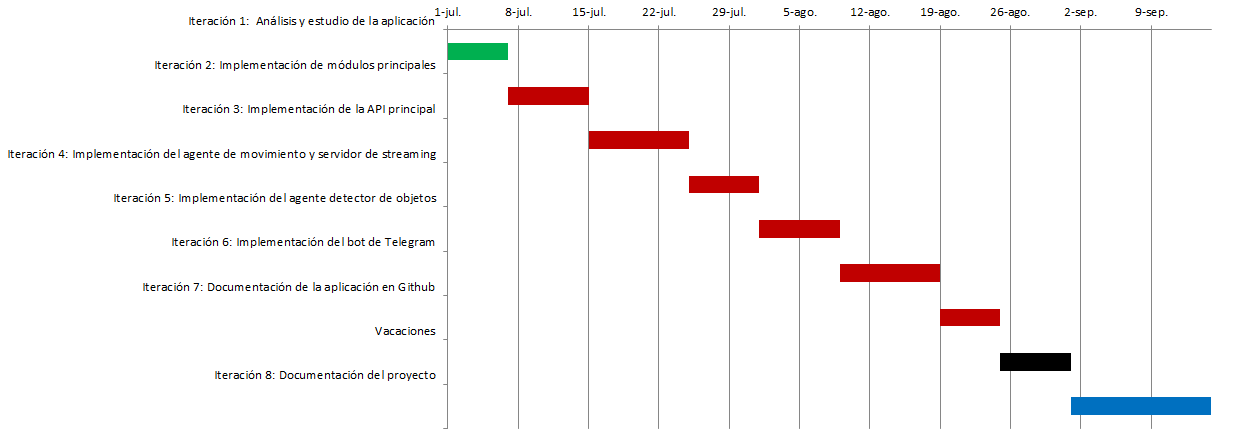
\includegraphics[scale=0.45]{images/diagrama_gantt}
	\caption{Diagrama de Gantt del proyecto}
\end{figure}

En la sección \ref{sec:conclusiones} (conclusiones y trabajos futuros), se realizará una pequeña comparativa entre este diagrama de Gantt y el que realmente se ha obtenido tras el desarrollo del proyecto.